\section{Versuchsaufbau und Versuchsdurchführung}

\begin{flushleft}
    Der Versuch wird wie in Abbildung \ref{Abbildung3} zu sehen geschaltet.
\end{flushleft}

\begin{figure}[H]
    \centering
    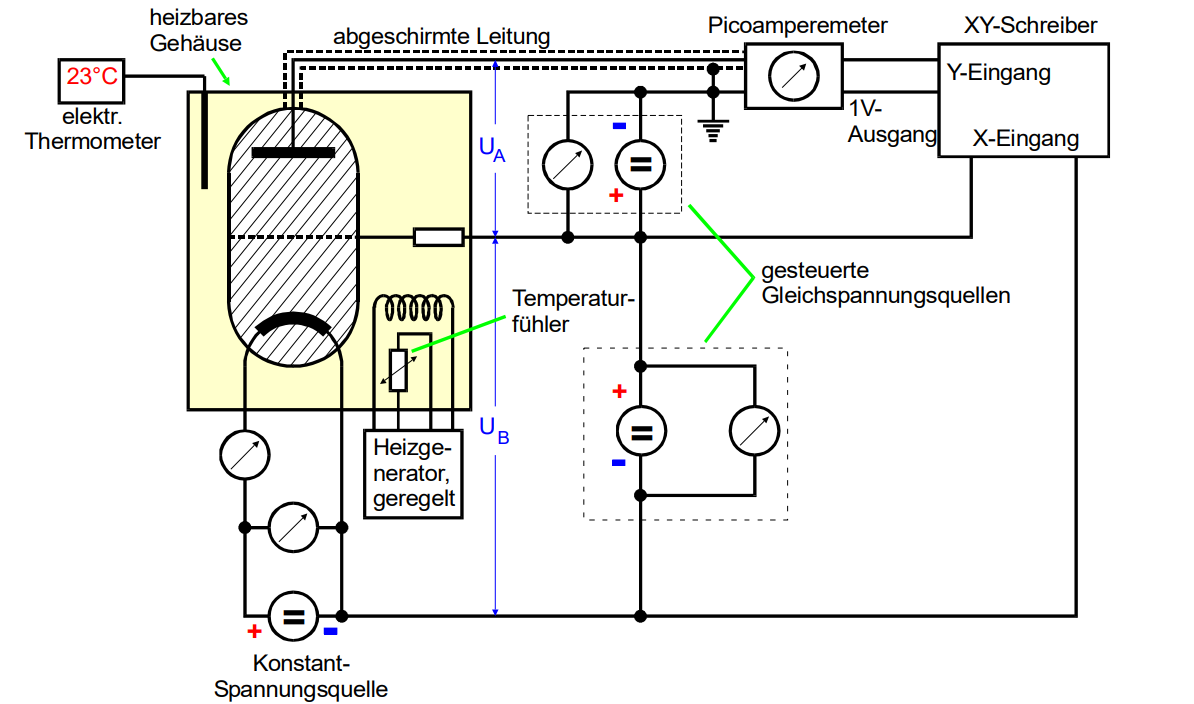
\includegraphics[height=75mm]{bilder/Ab3.png}
    \caption{Aufbau zur Aufnahme der Franck-Hertz-Kurve \cite{a1}. \label{Abbildung3} }
\end{figure}

\subsection{Bestimmung der Integralen Energieverteilung}

\begin{flushleft}
    Für die Bestimmung der integralen Energieverteilung wird die Beschleunigungsspannung auf $11\,\unit{\volt}$ gestellt.
    Bei Zimmertemperatur wird wird nun die Bremsspannung von $0\,\unit{\volt}$ auf $10\,\unit{\volt}$ kontinuierlich erhöht.
    Auf dem XY-Schreiber wird der Verlauf folglich aufgezeichnet.
    Wiederholt wird dies für eine Temperatur von zwischen $24,4\unit{\celsius}$ und $148,9\unit{\celsius}$.
    Beide Aufnahmen werden auf einem Papier gemacht, um den Verlauf bzw. die Unterschiede besser beobachten zu können.
\end{flushleft}

\subsection{Aufnahme der Franck-Hertz-Kurven}

\begin{flushleft}
Bei der Aufnahme der Franck-Herz-Kurve wird der Beschleunigungsraum auf eine Temperatur $178,9\unit{\celsius}$  erhitzt.
Danach wird die Beschleunigungsspannung von $0\,\unit{\volt}$ auf $60\,\unit{\volt}$ kontinuierlich erhöht.
Dieser Bereich kann aber je nach gewählter Temperatur kleiner gewählt werden um gute Aufnahmen zu erhalten.
Dies wird erneut auf dem XY-Schreiber festgehalten und für eine weitere Temperatur von $182,3\unit{\celsius}$.
\end{flushleft}